\section{Methodische Vorgehensweise}
Der Forschungsbereich dieser wissenschaftlichen Abhandlung umfasst die Themengebiete CI/CD sowie CEA. Da in Kombination dieser beiden Forschungsbereiche sowie in der praktischen Umsetzung dieser Konzepte mit SAP-spezifischen Technologien in der Literatur kein Datenmaterial vorhanden ist, werden im Rahmen dieser Arbeit Experteninterviews durchgeführt. Zur Analyse und Bewertung der CI/CD-Tools wird das AHP-Verfahren angewandt. Dabei sollen die in den Gesprächen erhobenen Daten als Entscheidungsgrundlage zur Durchführung des Analyseverfahrens verwendet werden. 
\subsection{Semistrukturierte Leitfadeninterviews zur Erhebung qualitativer Daten}
Das Experteninterview stellt eine häufig angewandte Analysemethode dar, welche vorrangig bei qualitativen Untersuchungen verwendet wird. Die Meinungen, Erfahrungen und Perspektiven der Experten werden dazu verwendet, relevante Aspekte zu einem Thema zu identifizieren oder eine Forschungshypothese zu formulieren. Diese wissenschaftliche Methode wird dabei insbesondere für aktuelle, stets unerforschte Themen sowie Fragestellungen mit geringem Literaturaufkommen verwendet \cite[S. 33 ff.]{Kaiser.2021}. Als Experten werden in diesem Zusammenhang Interviewpartner bezeichnet, welche aufgrund ihres im Rahmen beruflicher Tätigkeiten erworbenen Wissens umfassende Kenntnisse in einem spezifischen Fachgebiet besitzen. In der Literatur werden verschiedene Arten von Experteninterviews definiert. Dazu gehören \textit{strukturierte}, \textit{semistrukturierte} sowie \textit{unstrukturierte Interviews} \cite[S. 84 ff.]{Kaiser.2021}. Strukturierte Interviews zeichnen sich dabei insbesondere durch die Vorabfestlegung der im Interview gestellten Fragen aus. Hierbei wird bezweckt, dass allen Teilnehmenden dieselben Fragen in standardisierter Reihenfolge vorgelegt werden \cite[S. 421 ff.]{Aghamanoukjan.2009}. Im anderen Extrem der unstrukturierten Interviews erfolgt lediglich eine Bestimmung des Gesprächthemas, jedoch werden vorab keine expliziten Fragen festgelegt \cite[S. 441 ff.]{Aghamanoukjan.2009}. Den konkreten Verlauf des Gespräches bestimmt dabei die dynamische Entwicklung des Antwort-Nachfrage-Verhaltens der Interviewteilnehmer. Aufgrund des eng abgegrenzten Forschungsbereichs, besteht bei der Durchführung von unstrukturierten Interviews in dieser Arbeit das Risiko, dass die Gesprächsinhalte vom eigentlichen Untersuchungsgegenstand abweichen. Auch die Abwicklung von strukturierten Interviews ist für diese Arbeit nicht geeignet. Das liegt insbesondere an dem starren Erhebungsdesign dieser Interviewform. Angesichts der in dieser Arbeit angestrebten Erschließung unerforschter Themengebiete bietet eine Vorabfestlegung der Fragen nicht genügend Flexibilität, um auf neu aufkommende Aspekte innerhalb des Gesprächs angemessen zu reagieren. Deshalb werden im Rahmen dieser Arbeit semistrukturierte Interviews durchgeführt. Diese Interviewform realisiert eine Leitfadenstruktur, welche eine vordefinierte Fragegestaltung vorgibt, jedoch im Verlauf des Gesprächs gleichzeitig ein hohes Maß an Flexibilität bietet. Ergeben sich während eines Expertengesprächs neue Aspekte, können diese mit unmittelbaren Ad-hoc-Fragen aufgegriffen werden. Um die Interviews auszuwerten, muss eine Transkription der Expertengespräche erfolgen \cite[179]{Aghamanoukjan.2009}. Da zur Beantwortung der Forschungsfrage dieser Arbeit nicht der exakte Wortlaut, sondern vielmehr die inhaltliche Ausgestaltung der Expertengespräche von Bedeutung ist, wird eine zusammenfassende Transkription durchgeführt. Zur Auswertung der Transkription wird i.d.R. eine \textit{deduktive} bzw. \textit{induktive Methode} verwendet. Bei einer deduktiven Auswertung werden Aussagen der Experten vordefinierten Kategorien zugeordnet \cite[663]{Aghamanoukjan.2009}. Dieses Evaluationsverfahren bietet insbesondere zur Validierung einer vorabdefinierten Forschungshypothese einen erheblichen Mehrwert. Da im Rahmen dieser Arbeit stattdessen die Beantwortung einer offenen Fragestellung vorgesehen ist, wird eine induktive Kodierung der Interviews vorgenommen. Statt Kategorien im Voraus festzulegen, werden diese bei der induktiven Kodierung dynamisch aus dem Interviewmaterial abgeleitet \cite[663]{Aghamanoukjan.2009}. Eine implizite Auswertung der induktiven Kodierung wird im AHP-Verfahren (s. Kap. \ref{sec:AHP}) angewendet. So werden die während der Evaluation getroffenen Entscheidungen anhand der Expertenaussagen referenziert.

\subsection{Evaluation von Integrations- und Bereitstellungs-Tools unter Anwendung des Analytischen Hierarchieprozesses}
\label{sec:meth_ahp}
AHP ist ein von dem Mathematiker Thomas Saaty konzipiertes Entscheidungs-Framework. Dieses Rahmenwerk eignet sich insbesondere für komplexe betriebswirtschaftliche und technische Entscheidungsprobleme. Bei AHP wird eine Bewertung der Entscheidungsalternativen anhand verschiedener Kriterien vorgenommen. Das zugrundeliegende Rahmenwerk basiert dabei auf der Prämisse einer divergierenden Wichtigkeit der unterschiedlichen Entscheidungskriterien. Diese Methode erweist sich also als besonders geeignet, wenn es erforderlich ist, eine Bewertung von Entscheidungsalternativen auf Präferenzen verschiedener Stakeholder abzustimmen \cite[86]{Saaty.2008}. Das AHP-Verfahren besteht dabei aus mehreren Schritten. Zu Beginn des AHP-Verfahrens ist eine exakte Definition der zu lösenden Problemstellung notwendig. Im nächsten Schritt werden verschiedene Entscheidungsalternativen sowie Bewertungskriterien festgelegt. Die Entscheidungsstruktur kann dabei beliebig durch einen hierarchischen Aufbau gestaltet werden (s. Abb. \ref{fig:AHP_B}). 
\begin{center}
	\begin{figure}[H]
		\centering
		\scalebox{0.3}{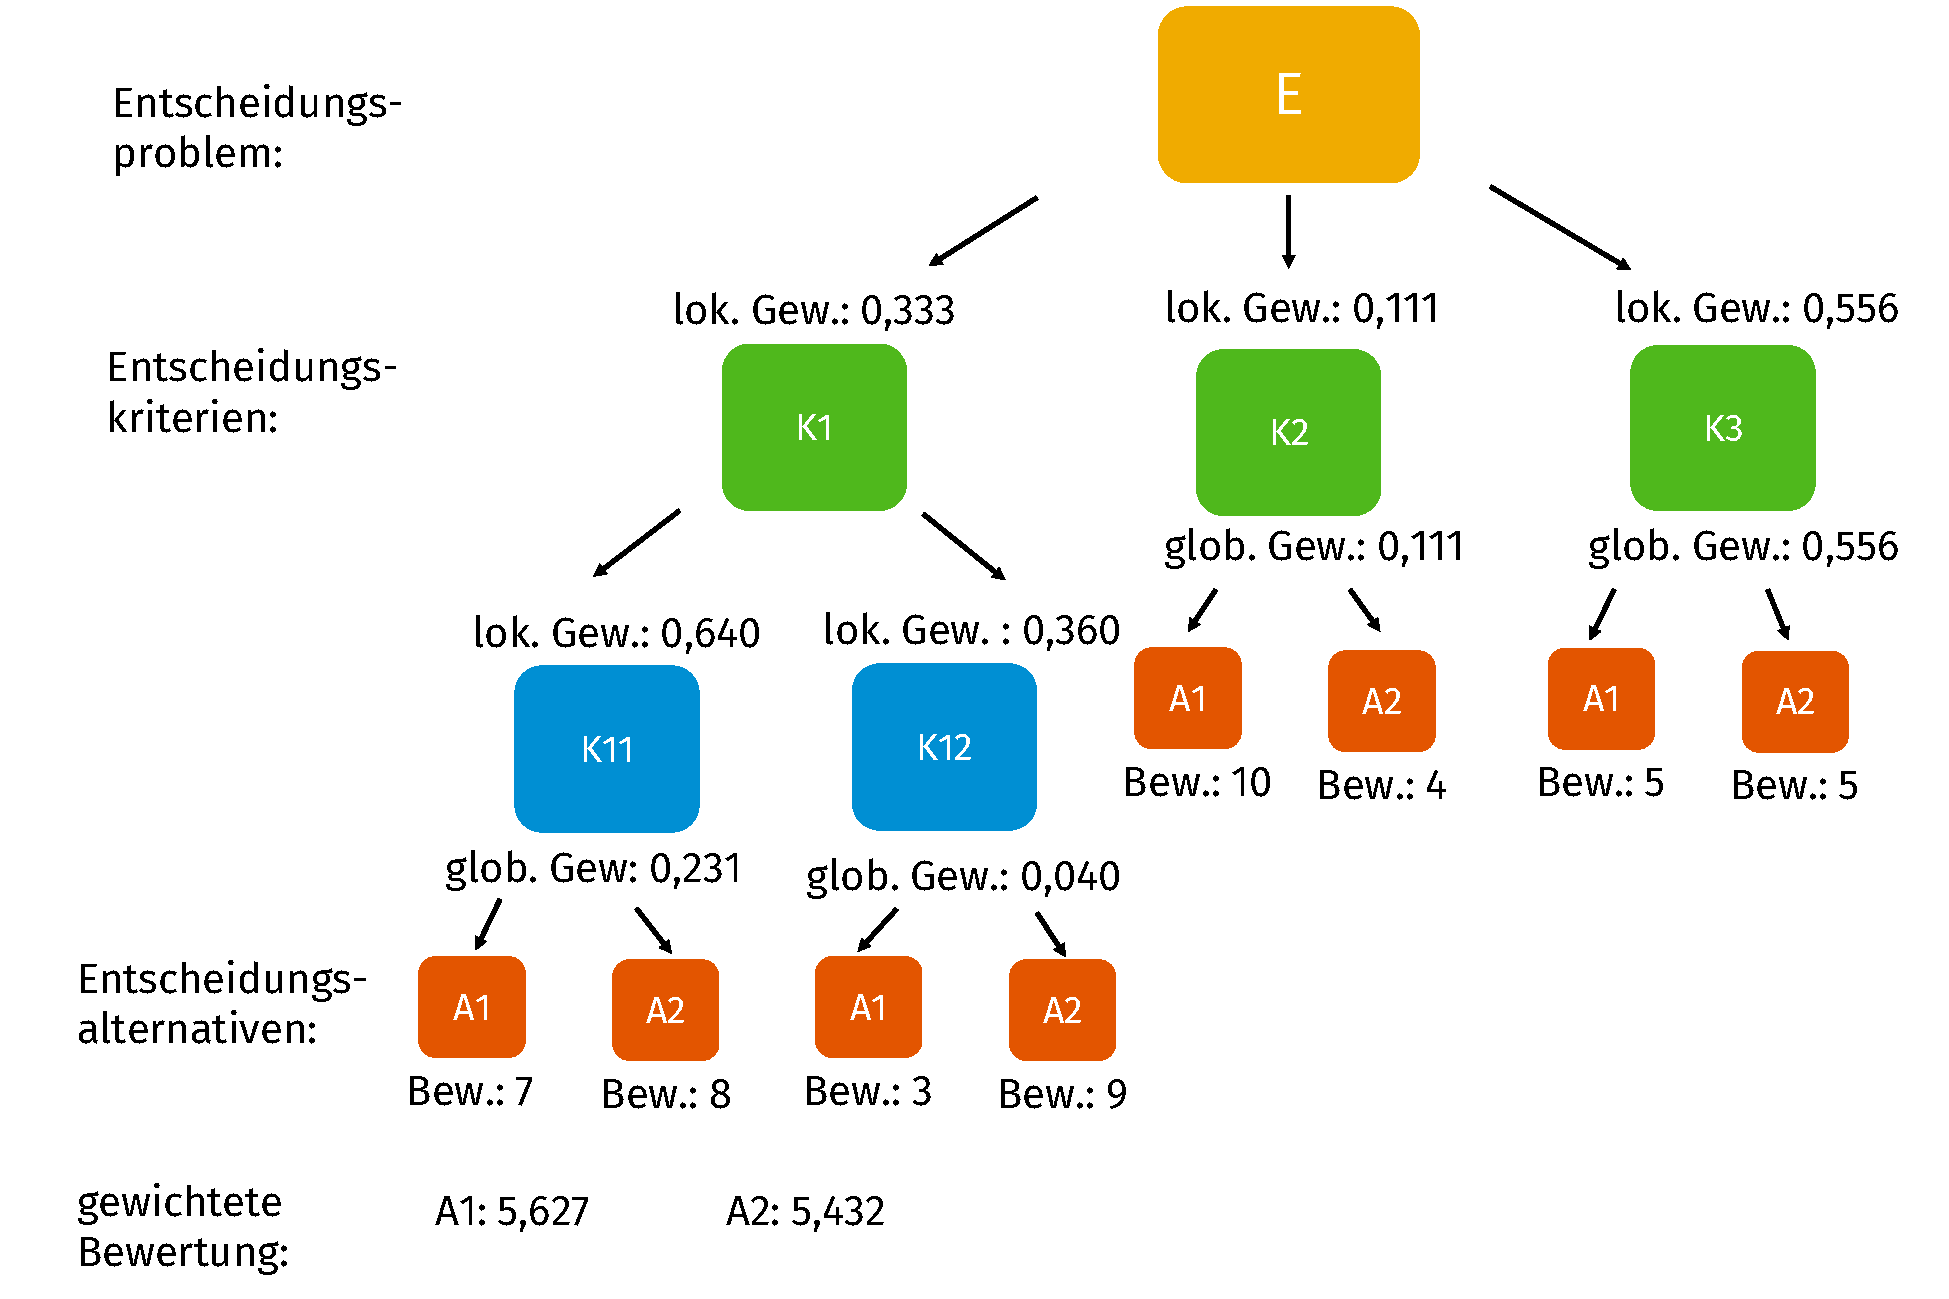
\includegraphics{AHP_H}}
		\caption[Exemplarische Darstellung der hierarchischen Entscheidungsstruktur im AHP]{Exemplarische Darstellung der hierarchischen Entscheidungsstruktur im AHP. Eigene Darstellung.}
		\label{fig:AHP_B}
	\end{figure}
\end{center}
\vspace*{-10mm}
Auf oberster Ebene des AHP-Baums befindet sich das Entscheidungsproblem. Es besteht die Möglichkeit, ein Kriterium in mehrere Subkriterien zu unterteilen. Auf unterster Ebene befinden sich schließlich die im Hinblick auf die festgelegten Evaluationskriterien zu bewertenden Entscheidungsalternativen \cite[86]{Saaty.2008}. Um eine auf die Präferenzen der Stakeholder abgestimmte Bewertung zu ermöglichen, müssen die zuvor festgelegten Entscheidungskriterien gewichtet werden. Besteht der AHP-Baum aus mehreren Stufen, erfolgt für jede Ebene zunächst eine isolierte Gewichtung. Zur Bestimmung der relativen Wichtigkeit ist für das AHP-Verfahren nach Saaty ein paarweiser Vergleich vorhergesehen. Hierbei wird die Wichtigkeit eines Kriteriums gegenüber eines Anderen ermittelt. Die in der Literatur aufgeführte Gegenüberstellung erfolgt dabei auf einer Skala von eins bis neun \cite[86]{Saaty.2008}. Um den Prozess der Entscheidungsfindung für die Probanden intuitiver zu gestalten, wird von der in der Literatur etablierten Vorgehensweise abgewichen und eine eigene Methode konzipiert. So ist im Rahmen dieser Arbeit eine Gewichtung von null bis zwei vorhergesehen. Während der Wert zwei impliziert, dass ein Entscheidungskriterium wesentlich wichtiger ist, wird mit dem Index eins eine gleiche Gewichtung ausgedrückt. Eine relative Wichtigkeit mit dem Wert null bedeutet in diesem Zusammenhang, dass ein Kriterium weniger wichtig als die Vergleichskategorie ist.  
\begin{center}
	\begin{table}[H]
		\centering
		\scalebox{0.20}{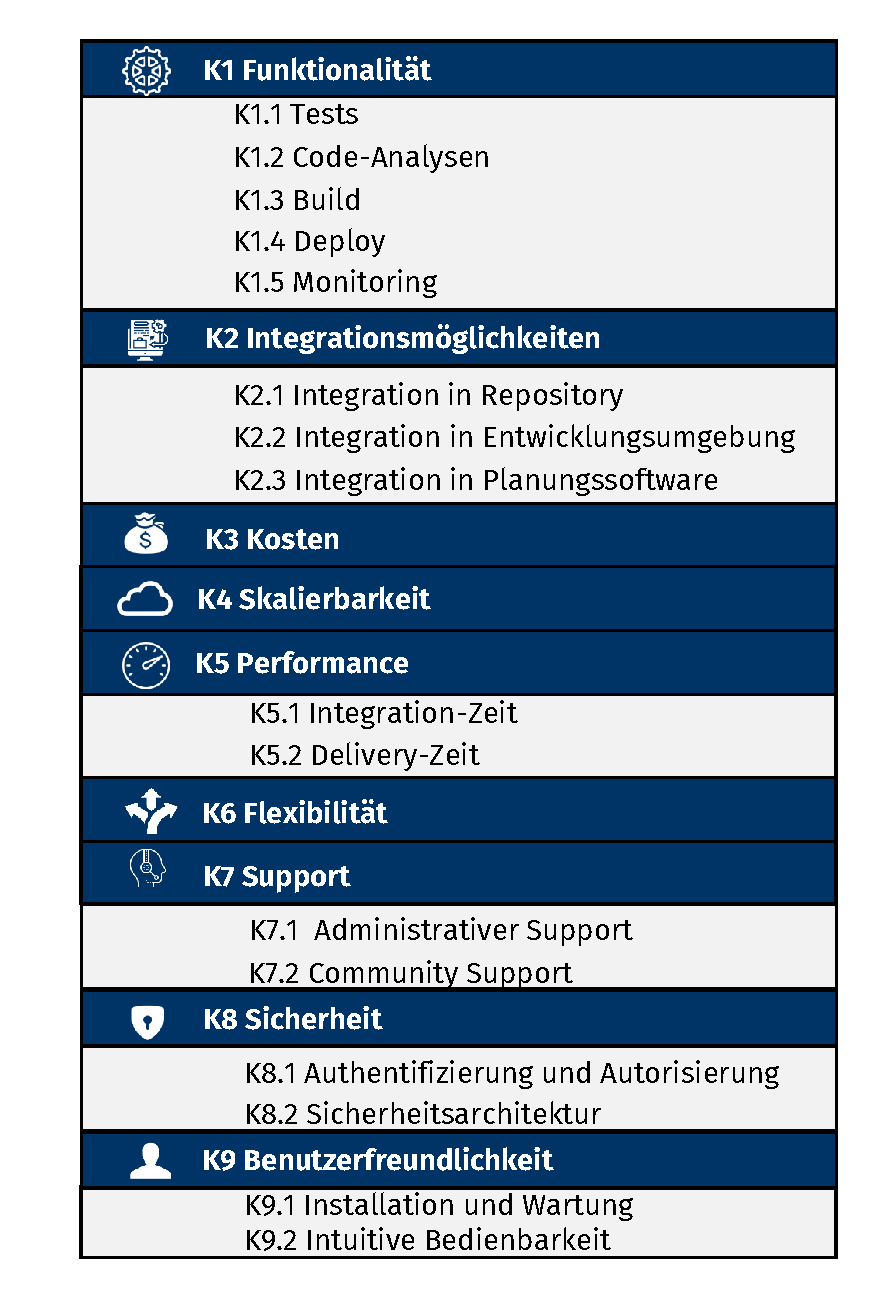
\includegraphics{AHP_B}}
		\caption[Exemplarische Darstellung der Paarvergleichsmatrix im AHP]{Exemplarische Darstellung der Paarvergleichsmatrix im AHP.\\ Eigene Darstellung.}
		\label{fig:AHP_B}
	\end{table}
\end{center}
\vspace*{-15mm}
So wird dem in Abb. \ref{fig:AHP_B} exemplarisch dargestellten Kriterium K1 eine wesentlichere Bedeutung als K2 zugeschrieben. Das korrespondiere Äquivalent auf der rechten Matrixhälfte besitzt entsprechend eine Gewichtung von null (\textit{weniger wichtig}). Um die Zuverlässigkeit der Paarvergleichsgewichtungen zu gewährleisten ist, für das AHP in der Literatur die Berechnung eines Konsitenzindex vorgesehen. Angesichts des hohen Zeitaufwands, welchen die Überprüfung transitiver Beziehungen bei der Durchführung der Gewichtung durch die Experten erfordern würde, wurde auf eine derartige Analyse im Rahmen dieser Arbeit verzichtet. Um der in der Paarvergleichsmatrix getroffenen Gegenüberstellung eine höhere Aussagekraft zu verleihen, müssen die relativen Gewichtungen in prozentuale Werte transformiert werden. Im ersten Schritt werden dabei alle Paarvergleichswerte eines Entscheidungskriteriums aufsummiert:\\
 \vspace{-6mm}
 \begin{center}
	$V_{ki}$ = $X_{KiKj+1}+X_{KiKj+2}+X_{KiKj+n}$	
 \end{center}
Anschließend muss diese Summe standardisiert werden. Hierfür wird die Gewichtungssumme ($V_{Ki}$) eines Kriteriums durch die Gesamtanzahl der in einer Paarvergleichsmatrix (\textit{N}) vergebenen Punkte dividiert. Diese ergibt sich durch die Anzahl der Kriterien (n) einer Paarvergleichsmatrix:
\vspace{-2mm}
\begin{center}
   $N$ = $ n \cdot n $	
\end{center}
Anschließend kann die prozentuale Gewichtung eines Entscheidungskriteriums wie folgt berechnet werden:
 \vspace{-2mm}
 \begin{center}
	$W_{ki}$ = $\frac{V_{Ki}}{N}$	
 \end{center}
Diese lokale Gewichtung wird für jede Hierarchieebene durchgeführt \cite[14341
]{Ishizaka.2011}. Um die globale Gewichtung ($P_{ki}$) zu ermitteln, wird die Gewichtung jedes Subkriteriums mit den Gewichtungen der übergeordneten Kriterien multipliziert :
\vspace{-2mm}
 \begin{center}
	$P_{Ki}$ = $W_{K1} \cdot W_{K2} \cdot W_{K3} \cdot W_{Kn} $	
 \end{center}
In der Literatur wird vorgesehen, dass auf unterster Hierarchieebene ebenfalls eine Gewichtung der Entscheidungsalternativen vorgenommen wird, um eine Bewertung durchzuführen \cite[88]{Saaty.2008}. Da dies insbesondere bei auf subjektiven Präferenzen basierenden Problemstellungen eine wichtige Rolle spielt, wird hierbei von dem Leitfaden nach Saaty abgewichen. Stattdessen wird für jedes Kriterium auf unterster Ebene eine feste Metrik definiert, anhand welcher die Alternativen bewertet werden. Letztlich werden die für jedes Kriterium erzielten Punkte mit den globalen Gewichtungsfaktoren multipliziert und alle Teilbewertungen zu einer gewichteten Gesamtbenotung zusammengezogen. Die Entscheidungsalternative mit der höchsten Gesamtbewertung gilt dabei als optimales Modell. 
Das Rahmenwerk eignet sich aufgrund des multidimensionalen Entscheidungsmodells besonders für die in der Arbeit zu untersuchenden Fragestellung. Die bei der Wahl einer CI/CD-Pipeline zu berücksichtigenden Aspekte können somit als Bewertungskriterien in den AHP-Baum aufgenommen werden. Des Weiteren ermöglicht die im AHP-Verfahren abgewickelte Gewichtung, dass die Kriterien in unterschiedlichem Maße Einfluss auf die Bewertung einer Pipeline nehmen. Im Rahmen dieser Arbeit kann somit die Wichtigkeit der an die Entscheidung geknüpften Aspekte durch verschiedene an der Bereitstellung von Software beteiligten Stakeholder (Entwickler, DevOps-Spezialisten etc.) festgelegt werden (s. Kap. \ref{sec:Gewichtung}). Dies ermöglicht eine auf die Präferenzen der Entscheidungsträger abgestimmte Bewertung der zu untersuchenden Pipelines. Das AHP-Verfahren besitzt darüber hinaus ebenfalls einen Vorteil bezüglich des Bewertungsdesigns. Während bei Methoden wie der SWOT-Analyse ausschließlich qualitative Aspekte berücksichtigt werden, ermöglicht das AHP-Model ebenfalls eine Evaluation quantitativer Bewertungsmetriken. Infolgedessen kann die Definition der Bewertungsmetrik flexibel und in Abhängigkeit des Entscheidungskriteriums getroffen werden. Im Rahmen dieser Arbeit wird anhand des AHP-Verfahrens ein für CEA optimales CI/CD-Tool bestimmt. Dabei ist jedoch zu beachten, dass bei der Wahl einer CI/CD-Pipeline ebenfalls \enquote{K.O.-Kriterien} existieren können, welche dazu führen, dass das Rahmenwerk für die Entscheidung keine relevante Aussagekraft mehr besitzt. Deshalb werden bei der Entwicklung der Handlungsempfehlung (s. Kap. \ref{sec:Handlungsempfehlung}) Szenarien definiert, bei welchen die Wahl der CI/CD-Pipeline vom AHP-Ergebnis abweicht. Weitere Erläuterungen zu den im AHP-Verfahren getroffenen Entscheidungen werden zur besseren Verständlichkeit in Kapitel \ref{sec:AHP} ausgeführt. 